\usetikzlibrary{calc}

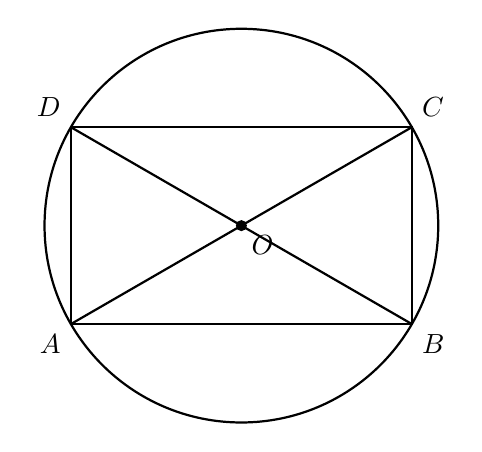
\begin{tikzpicture}[thick]

% Circle radius
\def\r{2.5}

% Center
\coordinate (O) at (0,0);

% Draw circle
\draw (O) circle (\r);

% Square vertices using angles on circle
\coordinate (A) at (210:\r);
\coordinate (B) at (330:\r);
\coordinate (C) at (30:\r);
\coordinate (D) at (150:\r);

% Draw square
\draw (A) -- (B) -- (C) -- (D) -- cycle;

% Draw diagonals
\draw (A) -- (C);
\draw (B) -- (D);

% Center dot
\fill (O) circle (2pt);

% Labels
\node[below left]  at (A) {$A$};
\node[below right] at (B) {$B$};
\node[above right] at (C) {$C$};
\node[above left]  at (D) {$D$};
\node[below right] at (O) {$O$};

\end{tikzpicture}